\documentclass[12pt,]{article}
\usepackage[left=1in,top=1in,right=1in,bottom=1in]{geometry}
\newcommand*{\authorfont}{\fontfamily{phv}\selectfont}
\usepackage[]{mathpazo}


  \usepackage[T1]{fontenc}
  \usepackage[utf8]{inputenc}




\usepackage{abstract}
\renewcommand{\abstractname}{}    % clear the title
\renewcommand{\absnamepos}{empty} % originally center

\renewenvironment{abstract}
 {{%
    \setlength{\leftmargin}{0mm}
    \setlength{\rightmargin}{\leftmargin}%
  }%
  \relax}
 {\endlist}

\makeatletter
\def\@maketitle{%
  \newpage
%  \null
%  \vskip 2em%
%  \begin{center}%
  \let \footnote \thanks
    {\fontsize{18}{20}\selectfont\raggedright  \setlength{\parindent}{0pt} \@title \par}%
}
%\fi
\makeatother




\setcounter{secnumdepth}{0}

\usepackage{longtable,booktabs}



\title{Political Donor Polarization  }



\author{\Large Ross Dahlke\vspace{0.05in} \newline\normalsize\emph{}  }


\date{}

\usepackage{titlesec}

\titleformat*{\section}{\normalsize\bfseries}
\titleformat*{\subsection}{\normalsize\itshape}
\titleformat*{\subsubsection}{\normalsize\itshape}
\titleformat*{\paragraph}{\normalsize\itshape}
\titleformat*{\subparagraph}{\normalsize\itshape}





\newtheorem{hypothesis}{Hypothesis}
\usepackage{setspace}


% set default figure placement to htbp
\makeatletter
\def\fps@figure{htbp}
\makeatother

\usepackage{graphicx}

% move the hyperref stuff down here, after header-includes, to allow for - \usepackage{hyperref}

\makeatletter
\@ifpackageloaded{hyperref}{}{%
\ifxetex
  \PassOptionsToPackage{hyphens}{url}\usepackage[setpagesize=false, % page size defined by xetex
              unicode=false, % unicode breaks when used with xetex
              xetex]{hyperref}
\else
  \PassOptionsToPackage{hyphens}{url}\usepackage[draft,unicode=true]{hyperref}
\fi
}

\@ifpackageloaded{color}{
    \PassOptionsToPackage{usenames,dvipsnames}{color}
}{%
    \usepackage[usenames,dvipsnames]{color}
}
\makeatother
\hypersetup{breaklinks=true,
            bookmarks=true,
            pdfauthor={Ross Dahlke ()},
             pdfkeywords = {},  
            pdftitle={Political Donor Polarization},
            colorlinks=true,
            citecolor=blue,
            urlcolor=blue,
            linkcolor=magenta,
            pdfborder={0 0 0}}
\urlstyle{same}  % don't use monospace font for urls

% Add an option for endnotes. -----


% add tightlist ----------
\providecommand{\tightlist}{%
\setlength{\itemsep}{0pt}\setlength{\parskip}{0pt}}

% add some other packages ----------

% \usepackage{multicol}
% This should regulate where figures float
% See: https://tex.stackexchange.com/questions/2275/keeping-tables-figures-close-to-where-they-are-mentioned
\usepackage[section]{placeins}


\begin{document}
	
% \pagenumbering{arabic}% resets `page` counter to 1 
%
% \maketitle

{% \usefont{T1}{pnc}{m}{n}
\setlength{\parindent}{0pt}
\thispagestyle{plain}
{\fontsize{18}{20}\selectfont\raggedright 
\maketitle  % title \par  

}

{
   \vskip 13.5pt\relax \normalsize\fontsize{11}{12} 
\textbf{\authorfont Ross Dahlke} \hskip 15pt \emph{\small }   

}

}








\begin{abstract}

    \hbox{\vrule height .2pt width 39.14pc}

    \vskip 8.5pt % \small 

\noindent American politics has recently been defined by unprecedented levels of
partisan polarization. Given the concurrent rise of the amount of money
in politics, many have suggested a connection between money in politics
and polarization. However, it remains unclear if donors have become more
polarized. Using political donation data from the Wisconsin Campaign
Finance Information System (CFIS) and the network science measure of
modularity, this paper shows that political donor networks have
polarized in the case study of Wisconsin. This polarization appears to
be connected to new donors, large donors, and donors from geographic
areas that are strong electorally for either party.


    \hbox{\vrule height .2pt width 39.14pc}


\end{abstract}


\vskip -8.5pt


 % removetitleabstract

\noindent \doublespacing 

\newpage

American politics is increasingly defined by polarization (Layman,
Carsey, and Horowitz 2006). Political polarization in America has
increased more than other countries around the world in the last four
decades (Boxell, Gentzkow, and Shapiro 2020). In addition, this
polarization is found at both at the elite and mass levels (Hare and
Poole 2014). Researchers have suggested a variety of potential causes of
polarization in the United States, including changing party composition,
growing racial divisions, the emergence of partisan cable news (Boxell,
Gentzkow, and Shapiro 2020), social media (Allcott et al. 2020; Tucker
et al. 2018), the form of American government (Pierson and Schickler
2020), and economic factors (Autor et al. 2020).

One other potential cause of polarization is political donors (Francia
et al. 2005). Political donors play an outsized role in American
politics. The amount of money spent and raised by political campaigns
continues to grow with every election cycle (Goldmacher 2020). The rise
in the amount of money in politics, along with a concurrent rise in
polarization, has led to the speculation that political donors are
contributors to polarization in politics (McCarty, Poole, and Rosenthal
2006). Barber (2016) concluded that ``the connection between donors and
candidates is an important part of the story of the polarization of
American politics.'' And while political donors do hold more extreme
policy positions than the public and partisan citizens (broockman2020;
Francia et al. 2005), it remains unanswered if political donors
themselves are polarizing.

I ask the question: \emph{Are political donors polarizing?}. To answer
this question, I build networks of political donors, where candidates
and donors are nodes and the donations connecting them are the edges, in
the 2010, 2012, and 2014 election cycles in Wisconsin state government
elections. Due to the attempted recall of the governor and members of
the state legislature, the state experienced three concurrent election
cycles with almost all of the same offices up for the election---a
rarity in American politics. In addition, many scholars and commentators
point to the attempted recall of then Governor Scott Walker as a
critical point in turning Wisconsin into one of the most polarized
states in the country.

This paper finds that political donors networks, compared to the 2010
election cycle, polarized during the 2012 election cycle and remained
polarized in the 2014 cycle. While this research does not attempt to
find any causal link between political donors and mass polarization, it
does suggest that political donors themselves have become more polarized
in time. In addition, the underlying data show potential connections
between donor polarization and new donors, large donors, and geographic
polarization in-line with electoral support.

\hypertarget{wisconsin-context}{%
\section{Wisconsin Context}\label{wisconsin-context}}

Both Wisconsin's legislators and mass public are among the most
polarized in the nation (Cramer 2016), and the state has been used by
academics to examine how political actions unfold in contentious and
highly divisive environment (Bode et al. 2018). Although many state
legislatures are also experiencing polarization (Shor 2015), Wisconsin
is unique in that there is a single event that many point to in creating
``the most politically divisive place in America'' (Kaufman 2012).

In 2011, newly-elected Republican Governor Scott Walker introduced Act
10,a highly inflamitory measure which scholars credit for inciting mass
polarization in the state. Act 10 was a ``budget reconciliation bill''
that stripped public school teachers of collective bargaining via their
union. Up to 100,000 people protested this ``anti-union bill'' at the
State Capitol and even occupied the capitol building for a period of
time (Sewell 2011). Democratic lawmakers fled to Illinois in an effort
to delay or stop the bill from passing into law (Layton 2011). In 2012
there was an unsuccessful election to recall Governor Walker.

Wisconsin Governor Scott Walker's self-anointed ``divide and conquer''
politics (Blake 2012) has left a political divide in Wisconsin that
persists to today. The result is that ``divisive politics ruled
Wisconsin over the last decade'' (Marley and Beck 2019). The Marquette
Law School poll headed by Charles Franklin has called public opinion in
Wisconsin a ``lesson in the two worlds of Wisconsin'' where ``it seems
often as if people have not only differing opinions but differing views
of facts and realities'' (Borsuk 2017).

This discrete event and its long-lasting consequences provides a unique
opportunity to study massively polarized politics that can be attributed
back to a single event. In addition, Wisconsin is a competitive swing
state that reflects a roughly 50-50 split similar to the country as a
whole.

\hypertarget{methodology-results}{%
\section{Methodology \& Results}\label{methodology-results}}

All data on political contributions came from the Wisconsin Campaign
Finance Information System (``Wisconsin Campaign Information System,''
n.d.). I exported all contributions to State Assembly, State Senate, and
Gubernatorial races from the 2010, 2012, and 2014 elections. This
dataset does not include donations to party committees, although it does
include disbursements from these committees. I manually created a table
of the parties of each of all the campaigns receiving contributions in
this timeframe and added the party of the campaign receiving the
donation to this dataset.

To clean and analyze my data I used the statistical programming language
R (R Core Team 2013; Wickham et al. 2019). I started with 1,499,603
donations. I then filtered out 3,503 unitemized/ anonymous donations,
removed punctuation from the names of the donors, and used Open Refine
(Kelli 2013) via the \texttt{refinr} R package (Muir 2018) to
standardize names (for example, Jim versus James). Next, I created a
unique identifier for donors by combining their standardized name with
their zip code. This identifier was created to be able to link donors
who contributed across multiple campaigns in multiple years without
considering two different people, with the same name, from different
locations to be the same person. Identity resolution is notoriously
difficult and is the biggest limitation of this paper. This study uses
some of the most advanced identity resolution techniques available, but
there is always inevitable error. While this potential error is
difficult to calculate, we expect that any error would be random
distributed across the three election cycles. In other words, one can
assume that the levels of error are the same across all three election
cycles. So, the directional conclusions of this paper remain valid.

Next, I estimated the partisanship of each donor in each election cycle
by taking the percent of donations that each donor gave to Republicans
divided by their donations to Republicans and Democrats. I took that
``percent donated to Republicans'' and rescaled it from -1 to 1, where
-1 represents the most Democratic donors, and 1 the most Republican
donors. I also calculated each individual's party bin based on the party
that they contributed a majority of their money to.

To quantify the levels of polarization in each election cycle, I
calculated two statistics: network modularity and average absolute
partisanship of donors.

First, political donations can be thought of as a network where donors
and candidates are nodes and donations connecting donors and candidates
are edges. This conceptualization of the political donor landscape as
network allows us to examine the network structure and calculate network
statistics on the graph of donors and candidates. One of the most useful
network statistics for measuring polarization in a network is modularity
(Newman 2006).

The modularity of a graph measures the strength of the division of
groups (such as political parties) by calculating ``the number of edges
falling within groups minus the expected number in an equivalent network
with edges placed at random'' (Newman 2006). The modularity of a network
falls in the range {[}-1/2, 1{]}. If the modularity is positive, the
number of edges that remain within each group is greater than the
expected number to remain in-group based on chance. The higher the
modularity, the greater the concentration of edges within each groups.
In other words, the higher the modularity of a network, the higher the
polarization among the groups. Formally, the equation to calculate
modularity Q is:

\[Q = \frac{1}{2m} \sum_{ij}\left[A_{ij} - \frac{k_{i}k_{j}}{2m} \right]\delta(g_{i},g_{j})\]

In this equation \(m = \frac{1}{2}\sum_{i}k_{i}\) is equal to the
strength of all the ties in the network, \(k_{i}=\sum_{j}A_{ij}\) is the
strength/ weighted degree of the \(i\)th node, \(g_{i}\) is the group
(in this case, party/ party bin) to which the \(i\) belong, and
\(\delta(g_{i},g_{j}) = 1\) if \(i\) and \(j\) belong to the same group
(party/ party bin) and 0 if they do not belong to the same party/ party
bin.

I calculated the modularity of the network graphs of each election cycle
(2010, 2012, 2014) using the \texttt{igraph} R package (Csardi and
Nepusz 2006). I used candidates' declared parties and donors' party bin
as the groups for the modularity calculation. The modularity of the
network graph of each election is in Table 1.

\begin{longtable}[]{@{}lr@{}}
\caption{Modularity calculation for the donor networks in each election
cycle. Higher modularity means more polarization.}\tabularnewline
\toprule
Election Cycle & Modularity\tabularnewline
\midrule
\endfirsthead
\toprule
Election Cycle & Modularity\tabularnewline
\midrule
\endhead
2010 & 0.41\tabularnewline
2012 & 0.49\tabularnewline
2014 & 0.48\tabularnewline
\bottomrule
\end{longtable}

In addition to calculating the change in modularity of each of the
election cycles, I also analyzed the change in mean absolute
partisanship of the donors in each election cycle (see Table 2).

I defined a donor's absolute partisanship as the absolute value of their
partisanship score (which is on a scale from -1 to 1). Therefore, the
larger a donor's absolute the partisanship, the higher percentage of
their money that they contributed to a single party. To calculate the
significance in the difference of the mean absolute partisanship, I use
a bootstrap methodology with 1,000 replications using the \texttt{infer}
R package (Bray et al. 2020). This paper uses a non-parametric
permutation method because of the non-Normal distribution of
partisanship of the donors (98\% of donors across all election cycles
only contribute to a single party).

\begin{longtable}[]{@{}lrll@{}}
\caption{Bootstrapped difference-in-means test with 1,000 replications
comparing mean partisanship of donors.}\tabularnewline
\toprule
Election Cycle & Diff. & CI & p\tabularnewline
\midrule
\endfirsthead
\toprule
Election Cycle & Diff. & CI & p\tabularnewline
\midrule
\endhead
2012 compared to 2010 & 0.04211 & 0.04025-0.04415 &
\textless.001\tabularnewline
2014 compared to 2012 & -0.00028 & -0.00089-0.00026 &
0.378\tabularnewline
\bottomrule
\end{longtable}

The results of this analysis show that political donors in Wisconsin
polarized during the 2012 election cycle. This phenomenon is best
visualized in Figure 1. This figure uses the Yifan Hu layout algorithm
(Hu 2005) in the Gephi software (Bastian, Heymann, and Jacomy 2009), a
force-directed graphical layout of networks that seeks to repulse
clusters of nodes from one another. The Yifan Hu layout algorithm is a
standard among social scientists studying networks such as online
networks (Adalat, Niazi, and Vasilakos 2018; Hemsley et al. 2015;
Khonsari et al. 2010; Rehman et al. 2020). This visual representation
shows two distinct clusters of donors (Democrats and Republicans) that
are reasonably close to one another in the 2010 election cycle and then
polarize significantly in the 2012 election cycle and remain polarized
in 2014. Table 3 includes the counts and percentages of that Democratic,
Republican, and bipartisan donors comprise of each election cycle.

\begin{figure}

{\centering \includegraphics[width=0.73\linewidth]{../figures/fig1} 

}

\caption{Visual representation of Wisconsin donor networks in the 2010, 2012 and 2014 election cycle using the Yifan Hu layout algorithm. Each dot/ node is a donor or campaign and lines/ edges connecting them are donations. Nodes sized by in-degree (incoming donations. Nodes and edges are colored by the partisanship of the donor. Percentages on the bars represent the percent of donors in each party bin.}\label{fig:unnamed-chunk-3}
\end{figure}

In addition, Figure 2 shows the partisan flow of political donors across
the election cycles, including the massive influx of new donors in both
the 2012 and 2014 election cycles. The counts and percentages of new and
old (donors who contributed in the last election cycle) are summarized
in Table 4.

\begin{figure}
\includegraphics[width=1\linewidth]{../figures/fig2} \caption{Sankey diagram of the flow of political donors in 2010, 2012, and 2014 election cycles in Wisconsin. The vertical bars are proportional to the number of donors in each bin.}\label{fig:unnamed-chunk-4}
\end{figure}

Figure 3 shows the partisan shift of donors who contributed in both the
2010 and 2012 election cycles.

\begin{figure}
\includegraphics[width=1\linewidth]{../figures/fig3} \caption{Every dot is a donor who contributed in 2010 and 2012. The bigger the dot, the more money they contribted. The x-axis is their partisanship in the 2010 election cycle and the y-axis is their partisanship in the 2012 election cycle. If the donor is to the right of the center diagonal line, they became more Republican. If they are to the left of the line, they became more Democratic.}\label{fig:unnamed-chunk-5}
\end{figure}

Figure 4 shows the distribution of the size of donors (amount
contributed) by partisanship.

\begin{figure}
\includegraphics[width=0.9\linewidth]{../figures/fig4} \caption{This box and whisker plot is grouped by the partisanship of the donors in the 2010 and 2012 election cycles. Note that the y-axis is shown on a log10 scale for clarity. The partisan distribution is shown along the bottom of the x-axis.}\label{fig:unnamed-chunk-6}
\end{figure}

Figure 5 is a map representing the geographic polarization among
political donors.

\begin{figure}
\includegraphics[width=0.9\linewidth]{../figures/fig5} \caption{This map shows the polarization of donor networks across Wisconsin's counties based on the net change of donors in each county per 10,000 residents. The red counties had a net increase in Republican donors, blue counties had a net increase for Democrats, and the purple counties had little or no change.}\label{fig:unnamed-chunk-7}
\end{figure}

Figure 6 shows the partisanship of donors in different geographic
categories. Table 3 is a table of the average partisanship of those
different geographic categories. Figure 7 is a graph of each county in
Wisconsin and the percentage of their vote for the Republican Scott
Walker for Governor in 2012 and the average percentage contributed to
Republicans in the 2012 cycle. These two measures, electoral and donor
partisanship in counties are significantly correlated (\emph{r} = 0.54,
\emph{p} = \textless.001).

\begin{figure}
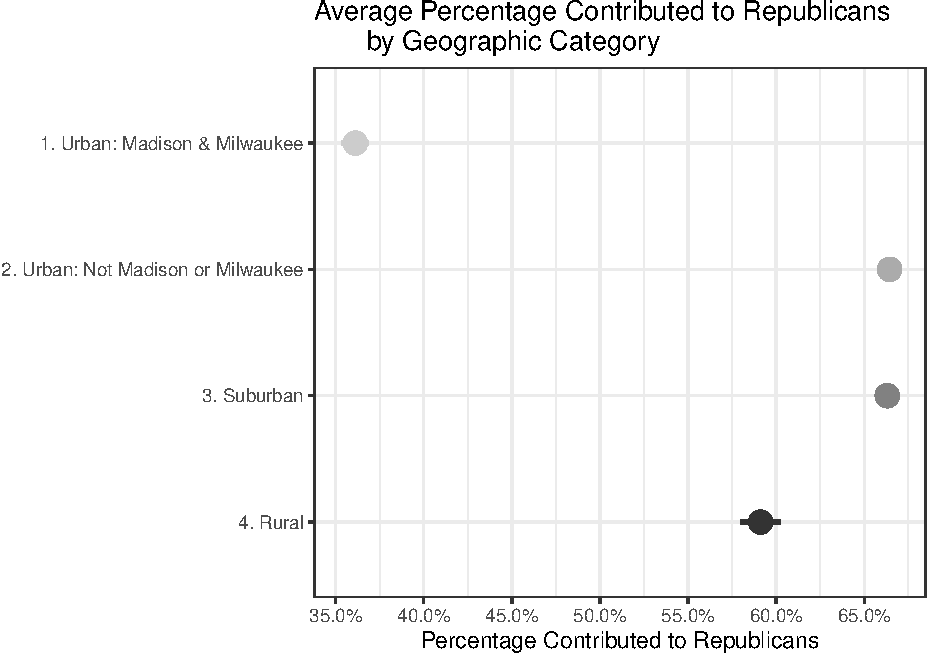
\includegraphics[width=1\linewidth]{output_only_files/figure-latex/unnamed-chunk-8-1} \caption{Average Percentage Contributed to Republican Candidates in Wisconsin in 2012 by Geography.}\label{fig:unnamed-chunk-8}
\end{figure}

\begin{longtable}[]{@{}llll@{}}
\caption{Average Percentage Contributed to Republicans by Geographic
Category}\tabularnewline
\toprule
Geographic Category & Avg. \% to Republicans & Low Estimate & High
Estimate\tabularnewline
\midrule
\endfirsthead
\toprule
Geographic Category & Avg. \% to Republicans & Low Estimate & High
Estimate\tabularnewline
\midrule
\endhead
1. Urban: Madison \& Milwaukee & 36.1\% & 35.3\% & 36.9\%\tabularnewline
2. Urban: Not Madison or Milwaukee & 66.4\% & 66.0\% &
66.8\%\tabularnewline
3. Suburban & 66.3\% & 65.7\% & 66.9\%\tabularnewline
4. Rural & 59.1\% & 58.0\% & 60.2\%\tabularnewline
\bottomrule
\end{longtable}

\begin{figure}
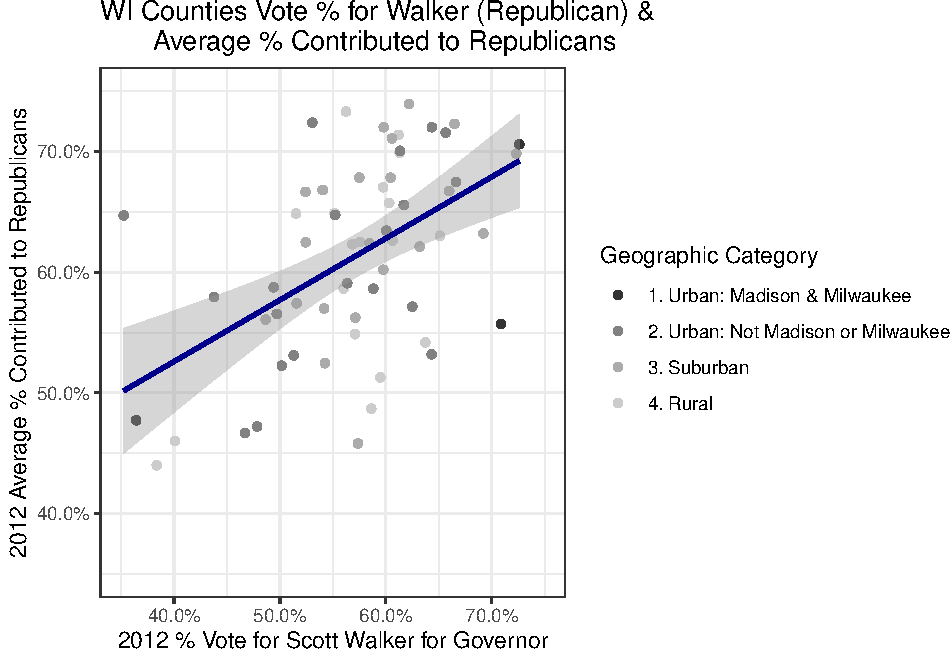
\includegraphics[width=1\linewidth]{output_only_files/figure-latex/unnamed-chunk-10-1} \caption{Wisconsin Counties 2012 percent vote for Scott Walker in the Gubernatorial Recall versus 2012 avergae percent contributed to Republican candidates.}\label{fig:unnamed-chunk-10}
\end{figure}

\hypertarget{discussion}{%
\section{Discussion}\label{discussion}}

The results of this paper show that political donor networks polarized
between the 2010 and 2012 election cycles and remained polarized in the
2014 cycle, as visualized in Figure 1. Further, during the time period
of polarization, there was a large influx of new donors, existing donors
polarized, small and large donors in polarized positions, and geographic
patterns emerged that are similar to electoral bases of support.

\hypertarget{new-donors}{%
\subsection{New Donors}\label{new-donors}}

Figure 2 shows that new donors overwhelmed the donorate in the 2012 and
2014 election cycles. The polarizing event of the attempted recall of
then Governor Walker potentially spurred this growth in new donors.
Previous research by Oklobzija (2016) reached a similar conclusion that
``politically polarizing events bear dividends for extremist lawmakers''
in California who raised more money as a result of polarizing political
events.

\hypertarget{existing-donors}{%
\subsection{Existing Donors}\label{existing-donors}}

In addition to new donor overwhelming the donor networks, donors that
contributed in both the 2010 and 2012 election cycles also showed
polarized behavior, as visualized in Figure 3. Previously bi-partisan
donors becoming single-party donors is very similar to the decreases in
split-ticket voting (Bump 2016; Desilver 2016; Skelley 2018).

\hypertarget{donor-sizes}{%
\subsection{Donor Sizes}\label{donor-sizes}}

Both large and small donors potentially play a role in the polarization
of donor networks and politics more broadly. Purely partisan donors were
the smallest donors, but then the next most partisan donors were on
average the largest donors. Further research should investigate the
differences in purely-partisan donors and nearly-partisan donors.
Potentially, these larger nearly-partisan donors are the ones who are
the most strategic in their contributions.

In addition, small-dollar donors are playing an increasing role in
campaign finance for both Democrats (Albert and Raja 2020) and
Republicans (Lott 2019). Although small-dollar donors were not as
prominent in the 2010, 2012, and 2014 state-level elections in Wisconsin
as recent national politics, they certainly played a role in the data of
this study. Figure 4 shows that 100\% partisan donors were on average
much small donors than non-100\% donors. Previous research into
small-dollar donors has asked, ``Are Small Donors Polarizing?'' and came
to the same conclusion as this paper of a more polarized politics as
potentially spurring the rise of small-dollar donors and not the other
way around (Keena and Knight-Finley 2019).

\hypertarget{donor-geography}{%
\subsection{Donor Geography}\label{donor-geography}}

Finally, a major theme of polarization studies is the rise of geographic
sorting. There has been ``an increased concentration of partisan
behavior'' that emphasizes ``a local residential spatial pattern of
geographic polarization'' (Kinsella, McTague, and Raleigh 2015).
``Partisan migrants'' are found to ``prefer to relocate in areas
populated with copartisans'' (Cho, Gimpel, and Hui 2012). The geography
of political polarization in Wisconsin is well-studied by Cramer (2016)
who uses the term ``urban-rural divide'' to explain the geographic
polarization of the state. This divide that Cramer documents across
Wisconsin manifests itself in the geography of polarization among
political donors (Figure 5). Although past research has suggested that
Democratic and Republican campaign contribution come from the same
geographic area (Bramlett, Gimpel, and Lee 2011), this paper, shown in
Figure 6 and Table 3, find different partisanship in donors in different
geographic areas.

Donors from Madison and Milwaukee are much less Democratic than other
urban areas and suburban areas, with rural areas inbetween. Further, the
partisanship of donors in a county is highly correlated to the electoral
partisanship of the county they are from, as seen in Figure 7. This
correlation suggests that the act of donating is becoming more aligned
with voting, and that geography is playing an increasing role in
politics.

\hypertarget{conclusion}{%
\section{Conclusion}\label{conclusion}}

This paper asked: \emph{Are political donors polarizing?}. In the case
of Wisconsin, this paper finds that political donor networks are
polarizing. During the time period of increasing polarization, there was
a massive influx of new donors, polarization of existing donors,
polarized small and large donors, and geographic patterns matching bases
of electoral support.

\newpage

\hypertarget{references}{%
\section*{References}\label{references}}
\addcontentsline{toc}{section}{References}

\hypertarget{refs}{}
\leavevmode\hypertarget{ref-adalat2018}{}%
Adalat, Mohsin, Muaz A. Niazi, and Athanasios V. Vasilakos. 2018.
``Variations in Power of Opinion Leaders in Online Communication
Networks.'' \emph{Royal Society Open Science} 5 (10).

\leavevmode\hypertarget{ref-albert2020}{}%
Albert, Zachary, and Raymond La Raja. 2020. ``Small Dollar Donors and
the Evolving Democratic Party.'' \emph{American Political Science
Association Preprints}.

\leavevmode\hypertarget{ref-allcott2020}{}%
Allcott, Hunt, Luca Braghieri, Sarah Eichmeyer, and Matthew Gentzkow.
2020. ``The Welfare Effects of Social Media.'' \emph{American Economic
Review} 110 (3): 629--76. \url{https://doi.org/10.1257/aer.20190658}.

\leavevmode\hypertarget{ref-autor2020}{}%
Autor, David, David Dorn, Gordon Hanson, and Kaveh Majlesi. 2020.
``Importing Political Polarization? The Electoral Consequences of Rising
Trade Exposure.'' \emph{American Economic Review} 110 (10): 3139--83.
\url{https://doi.org/10.1257/aer.20170011}.

\leavevmode\hypertarget{ref-barber2016a}{}%
Barber, Michael J. 2016. ``Ideological Donors, Contribution Limits, and
the Polarization of American Legislatures.'' \emph{The Journal of
Politics} 78 (1): 296--310.

\leavevmode\hypertarget{ref-gephi}{}%
Bastian, Mathieu, Sebastien Heymann, and Mathieu Jacomy. 2009. ``Gephi:
An Open Source Software for Exploring and Manipulating Networks.''
\url{http://www.aaai.org/ocs/index.php/ICWSM/09/paper/view/154}.

\leavevmode\hypertarget{ref-blake2012}{}%
Blake, Aaron. 2012. ``Scott Walker Said Budget Strategy in Wisconsin Was
'Divide and Conquer'.'' \emph{The Washington Post}, May.

\leavevmode\hypertarget{ref-bode2018}{}%
Bode, Leticia, Stephanie Edgerly, Chris Wells, Itay Gabay, Charles
Franklin, Lew Friedland, and Dhavan V. Shah. 2018. ``Participation in
Contentious Politics: Rethinking the Roles of News, Social Media, and
Conversation Amid Divisiveness.'' \emph{Journal of Information
Technology \& Politics} 15 (3): 215--29.

\leavevmode\hypertarget{ref-borsuk2017}{}%
Borsuk, Alan. 2017. ``New Poll Gives Vivid Look into Polarized Political
Perceptions.'' June 29, 2017.
\url{https://law.marquette.edu/poll/2017/06/29/new-poll-gives-vivid-look-into-polarized-political-perceptions/}.

\leavevmode\hypertarget{ref-boxell2020}{}%
Boxell, Levi, Matthew Gentzkow, and Jesse M Shapiro. 2020.
``Cross-Country Trends in Affective Polarization.'' Working Paper 26669.
Working Paper Series. National Bureau of Economic Research.
\url{https://doi.org/10.3386/w26669}.

\leavevmode\hypertarget{ref-bramlett2011}{}%
Bramlett, Brittany H., James G. Gimpel, and Frances E. Lee. 2011. ``The
Political Ecology of Opinion in Big-Donor Neighborhoods.''
\emph{Political Behavior} 33: 565--600.

\leavevmode\hypertarget{ref-infer}{}%
Bray, Andrew, Chester Ismay, Evgeni Chasnovski, Ben Baumer, Mine
Cetinkaya-Rundel, Simon Couch, Ted Laderas, et al. 2020. \emph{Infer:
Tidy Statistical Inference}.
\url{https://cran.r-project.org/web/packages/infer/index.html}.

\leavevmode\hypertarget{ref-bump2016}{}%
Bump, Philip. 2016. ``The Decline and Fall of Split-Ticket Voting,
Visualized.'' \emph{The Washington Post}, May.

\leavevmode\hypertarget{ref-cho2012}{}%
Cho, Wendy K. Tam, James G. Gimpel, and Iris S. Hui. 2012. ``Voter
Migration and the Geographic Sorting of the American Electorate.''
\emph{Annals of the Association of American Geographers} 103 (4):
856--70.

\leavevmode\hypertarget{ref-cramer2016}{}%
Cramer, K. J. 2016. \emph{The Politics of Resentment: Rural
Consciousness in Wisconsin and the Rise of Scott Walker}. Chicago
Studies in American Politics. University of Chicago Press.
\url{https://books.google.com/books?id=Rg2ZCwAAQBAJ}.

\leavevmode\hypertarget{ref-igraph}{}%
Csardi, Gabor, and Tamas Nepusz. 2006. ``The Igraph Software Package for
Complex Network Research.'' \emph{InterJournal} Complex Systems: 1695.
\url{http://igraph.org}.

\leavevmode\hypertarget{ref-desilver2016}{}%
Desilver, Drew. 2016. ``Split-Ticket District, Once Common, Are Now
Rare.'' \emph{Pew Research Center Fact Tank}, August.

\leavevmode\hypertarget{ref-francia2005}{}%
Francia, Peter L., John C. Green, Paul S. Herrnson, Lynda W. Powell, and
Clyde Wilcox. 2005. ``Limousine Liberals and Corporate Conservatives:
The Financial Constituencies of the Democratic and Republican Parties.''
\emph{Social Science Quarterly} 86 (4): 761--78.

\leavevmode\hypertarget{ref-goldmacher2020}{}%
Goldmacher, Shane. 2020. ``The 2020 Campaign Is the Most Expensive Ever
(by a Lot).'' \emph{The New York Times Magazine}, October.

\leavevmode\hypertarget{ref-hare2014}{}%
Hare, Christopher, and Keith T. Poole. 2014. ``The Polarization of
Contemporary American Politics.'' \emph{Polity} 46 (3): 411--29.
\url{https://doi.org/10.1057/pol.2014.10}.

\leavevmode\hypertarget{ref-hemsley2015}{}%
Hemsley, Bronwyn, Stephen Dann, Stuart Palmer, Meredith Allan, and Susan
Balandin. 2015. ```We Definitely Need an Audience': Experiences of
Twitter, Twitter Networks and Tweet Content in Adults with Severe
Communication Disabilities Who Use Augmentative and Alternative
Communication (Aac).'' \emph{Disability and Rehabilitation} 37 (17):
1531--42. \url{https://doi.org/10.3109/09638288.2015.1045990}.

\leavevmode\hypertarget{ref-yifanhu}{}%
Hu, Yifan. 2005. ``Efficient, High-Quality Force-Directed Graph
Drawing.'' \emph{Mathematica Journal} 10 (1): 37--71.

\leavevmode\hypertarget{ref-kaufman2012}{}%
Kaufman, Dan. 2012. ``How Did Wisconsin Become the Most Politically
Divisive Place in America?'' \emph{The New York Times Magazine}, May.

\leavevmode\hypertarget{ref-keena2019}{}%
Keena, Alex, and Misty Knight-Finley. 2019. ``Are Small Donors
Polarizing? A Longitudinal Study of the Senate.'' \emph{Election Law
Journal: Rules, Politics, and Policy} 18 (2): 132--44.

\leavevmode\hypertarget{ref-openrefine}{}%
Kelli, Ham. 2013. ``OpenReinfe (Version 2.5).'' \emph{Journal of the
Medical Library Association} 101 (3): 233--34.

\leavevmode\hypertarget{ref-khonsari2010}{}%
Khonsari, K. K., Z. A. Nayeri, A. Fathalian, and L. Fathalian. 2010.
``Social Network Analysis of Iran's Green Movement Opposition Groups
Using Twitter.'' In \emph{2010 International Conference on Advances in
Social Networks Analysis and Mining}, 414--15.

\leavevmode\hypertarget{ref-kinsella2015}{}%
Kinsella, Chad, Colleen McTague, and Kevin N. Raleigh. 2015. ``Unmasking
Geographic Polarization and Clustering: A Micro-Scalar Analysis of
Partisan Voting Behavior.'' \emph{Applied Geography} 62 (August):
404--19.

\leavevmode\hypertarget{ref-layman2006}{}%
Layman, Geoffrey C., Thomas M. Carsey, and Juliana Menasce Horowitz.
2006. ``PARTY Polarization in American Politics: Characteristics,
Causes, and Consequences.'' \emph{Annual Review of Political Science} 9
(1): 83--110.
\url{https://doi.org/10.1146/annurev.polisci.9.070204.105138}.

\leavevmode\hypertarget{ref-layton2011}{}%
Layton, Lyndsey. 2011. ``'Wisconsin 14' Group of Democratic Senators
Returns, Greeted by Thousands at Capitol.'' \emph{The Washington Post},
March.

\leavevmode\hypertarget{ref-lott2019}{}%
Lott, Maxim. 2019. ``Trump Campaign's Small-Dollar Donations Surge,
Marking Major Shift for Gop.'' \emph{Fox News}, August.

\leavevmode\hypertarget{ref-marley2019}{}%
Marley, Patrick, and Molly Beck. 2019. ``Divisive Politics Ruled
Wisconsin over the Last Decade.'' \emph{Milwaukee Journal Sentinel},
December.

\leavevmode\hypertarget{ref-mccarty2006}{}%
McCarty, Nolan, Keith T. Poole, and Howard Rosenthal. 2006.
\emph{Polarizaed America: The Dancedance of Ideology and Unequal
Riches}. Cambridge, Mass: MIT Press.

\leavevmode\hypertarget{ref-refinr}{}%
Muir, Chris. 2018. \emph{Refinr: Cluster and Merge Similar Values Within
a Character Vector}.
\url{https://cran.r-project.org/web/packages/refinr/index.html}.

\leavevmode\hypertarget{ref-newman2006}{}%
Newman, M. E. J. 2006. ``Modularity and Community Structure in
Networks.'' \emph{Proceedings of the National Academy of Sciences} 103
(23): 8577--82. \url{https://doi.org/10.1073/pnas.0601602103}.

\leavevmode\hypertarget{ref-oklobzija}{}%
Oklobdzija, Stan. 2016. ``Closing down and Cashing in: Extremism and
Political Fundraising.'' \emph{State Politics \& Policy Quarterly} 17
(2): 201--24.

\leavevmode\hypertarget{ref-pierson2020}{}%
Pierson, Paul, and Eric Schickler. 2020. ``Madison's Constitution Under
Stress: A Developmental Analysis of Political Polarization.''
\emph{Annual Review of Political Science} 23 (1): 37--58.
\url{https://doi.org/10.1146/annurev-polisci-050718-033629}.

\leavevmode\hypertarget{ref-r}{}%
R Core Team. 2013. \emph{R: A Language and Environment for Statistical
Computing}. Vienna, Austria: R Foundation for Statistical Computing.
\url{http://www.R-project.org/}.

\leavevmode\hypertarget{ref-rehman2020}{}%
Rehman, Ateeq Ur, Aimin Jiang, Abdul Rehman, Anand Paul, Sadia din, and
Muhammad Tariq Sadiq. 2020. ``Identification and Role of Opinion Leaders
in Information Diffusion for Online Discussion Network.'' \emph{Journal
of Ambient Intelligence and Humanized Computing}, January.

\leavevmode\hypertarget{ref-sewell2011}{}%
Sewell, Abby. 2011. ``Protesters Out in Force Nationwide to Oppose
Wisconsin's Anti-Union Bill.'' \emph{Los Angeles Times}, February.

\leavevmode\hypertarget{ref-shor2015}{}%
Shor, Boris. 2015. ``Polarization in American State Legislatures.'' In
\emph{American Gridlock: The Sources, Character, and Impact of Political
Polarization}, edited by James A. Thurber and AntoineEditors Yoshinaka,
203--21. Cambridge University Press.
\url{https://doi.org/10.1017/CBO9781316287002.011}.

\leavevmode\hypertarget{ref-skelley2018}{}%
Skelley, Geoffrey. 2018. ``Split-Ticket Voting Hit a New Low in 2018
Senate and Governor Race.'' \emph{FiveThirtyEight}, January.

\leavevmode\hypertarget{ref-tucker2018}{}%
Tucker, Joshua A, Andrew Guess, Pablo Barberá, Cristian Vaccari,
Alexandra Siegel, Sergey Sanovich, Denis Stukal, and Brendan Nyhan.
2018. ``Social Media, Political Polarization, and Political
Disinformation: A Review of the Scientific Literature.'' \emph{Political
Polarization, and Political Disinformation: A Review of the Scientific
Literature (March 19, 2018)}.

\leavevmode\hypertarget{ref-tidyverse}{}%
Wickham, Hadley, Mara Averick, Jennifer Bryan, Winston Chang, Lucy
D'Agostino McGowan, Romain François, Garrett Grolemund, et al. 2019.
``Welcome to the tidyverse.'' \emph{Journal of Open Source Software} 4
(43): 1686. \url{https://doi.org/10.21105/joss.01686}.

\leavevmode\hypertarget{ref-cfis}{}%
``Wisconsin Campaign Information System.'' n.d.
\url{https://cfis.wi.gov/\#}.





\newpage
\singlespacing 
\end{document}
